\subsection*{A deployed agent relays corrupted live database values}
To test whether the problem arises outside a benchmark, we ran Biomni~\citep{huang2026biomni}, an open-source biomedical agent,
against the live UniProt and PubChem APIs and altered one field of selected responses in transit with an intercepting proxy
(Methods). Biomni retrieved and processed records with its own code and tools; we changed only what the databases returned. Each
of 300 tasks ran once without corruption, once with an impossible value and once with a plausible value within 25\% of the true
one, for two models, with hypotheses registered in advance (OSF vq5cp).

The corrupted value reached the agent in 95--96\% of corrupted runs; in the remainder the agent answered through another route
and never requested the corrupted field. Impossible values were almost always caught: they were relayed in 5 of 287 runs with
DeepSeek~V4.1~Flash and 6 of 286 with Gemini~3.8~Flash. Plausible values were relayed in 28\% (80/285) and 24\% (69/288) of runs,
far fewer than in the controlled benchmark below (McNemar $p<10^{-30}$ for both models) but not rare.
% src: results/biomni_full_deepseek, results/biomni_full_flash (delivery 287/285 and 286/288; H1 tests)

Where plausible values were relayed contradicted our second prediction. We had expected fields with an exact derivation route to
be protected; instead they were relayed more often (odds ratio 5.6 and 3.6). Protein length and mass, which follow exactly from
the sequence, were relayed in 46--68\% of plausible runs, organism in 0--14\% and names in 0--8\%, and numeric chemistry fields
almost never, because Biomni's own workflow recomputes them with RDKit. A derivation route protected a value only when the agent's
workflow actually passed through it. A third prediction, about which concern an agent raises first, was supported for one model
and not the other (Supplementary Information).
% src: Biomni H2 per-field analysis; H3 results (DeepSeek p = 4e-5; Flash mixed)

\begin{figure}[t]
\centering
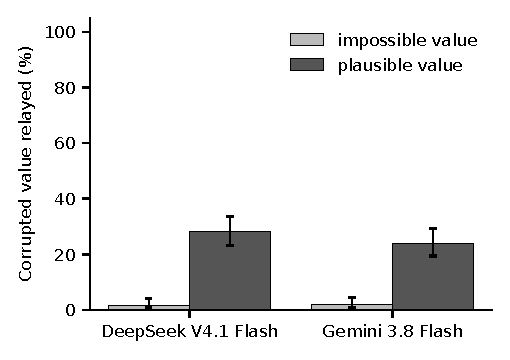
\includegraphics[width=\linewidth]{../figures/nmi_deployment.pdf}
\caption{\textbf{Study design and a deployed agent.} \textbf{a}, Corrupted values were injected between the database and the agent, in a tool layer or, for the deployed agent, an intercepting proxy; the agent's answer and concerns were scored. Bottom: the forms a corrupted record took (illustrative values). \textbf{b}, Biomni with live UniProt and PubChem APIs: share of corrupted runs in which the value was relayed, caught, or never requested (relayed/delivered at right). \textbf{c}, Relay of plausible values by field (95\% Wilson intervals).}
\label{fig:deploy}
\end{figure}
